\subsection{Global variables}
\begin{itemize}
	\item Global variables are defined anywhere outside of a function definition
	\item Space is set aside for these variables before the program begins execution, and is reserved for them until the program completes
	\item This space is reserved at compile time
	\item e.g.,
\begin{lstlisting}[style=C++]
const int SIZE=10;	// Global variable
int main() {
	//...
}
\end{lstlisting}
\end{itemize}

\subsection{Local variables}
\begin{itemize}
	\item Local variables are any variable defined within a block
	\item This includes function arguments, which act as if they were defined in the outermost block of the function
	\item Space is set aside for these variables when the relevant block is entered, and is reserved for them until the block is exited
	\item This space is reserved at run time, but the size is known to the compiler
	\item e.g.,
\begin{lstlisting}[style=C++]
int sum(int *array, int size) {
	int sum=0; 	// Local variable, alongside array (the pointer!) and size
	//...
}
\end{lstlisting}
\end{itemize}

\subsection{Dynamic variables}
\begin{itemize}
	\item It is dynamic because:
	\begin{itemize}
		\item Size (or number) is determined at runtime
		\item When it will be created and destroyed is determined at runtime
	\end{itemize}
\end{itemize}

\subsubsection{new}
\begin{itemize}
	\item Create dynamic variables using new
\begin{lstlisting}[style=C++]
int main() {
	int *p = new int;
}
\end{lstlisting}
	\item This creates new space for an integer, and returns a pointer to that space, assigning it to \lstinline[style=C++]{p}
	\item The initial value is undefined
	\item Use initializer syntax to assign an initial value:
\begin{lstlisting}[style=C++]
int main() {
	int *p = new int(5);
}
\end{lstlisting}
\end{itemize}

\subsubsection{delete}
\begin{itemize}
	\item Destroy dynamic variables using \lstinline[style=C++]{delete}
\begin{lstlisting}[style=C++]
int *p= new int;
//do something with p
delete p;
delete p; //Error!
\end{lstlisting}
	\item Releases the claim on the space previously used by the \lstinline[style=C++]{int}
	\item You can only \lstinline[style=C++]{delete} a dynamic variable \textit{once}
\begin{lstlisting}[style=C++]
delete p;
delete p; //Error!
\end{lstlisting}
	\item Assigning NULL to deleted pointers prevents this issue:
\begin{lstlisting}[style=C++]
delete p; p=0;
delete p; // Ok
\end{lstlisting}
	\item Only objects that are created with \lstinline[style=C++]{new} can be destroyed by \lstinline[style=C++]{delete}
\end{itemize}

\subsubsection{Dynamic array}
\begin{itemize}
	\item e.g.,
\begin{lstlisting}
//ask user to enter integer size
int size = get_size_from_user();

int *p= new int[size];
//do something with p ...
delete[] p;
\end{lstlisting}
\end{itemize}

\subsection{Memory leaks}
\begin{itemize}
	\item Dynamic variables live until the programmer destroys them using \lstinline[style=C++]{delete}
	\item This is true even if you ``forge'' the pointer to the object.
\begin{lstlisting}[style=C++]
int main() {
	int *p1 = new int(1);
	int *p2 = new int(2);
	p1 = p2;
}
\end{lstlisting}
	\begin{center}
		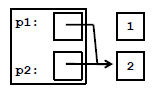
\includegraphics{sections/lec15/mem1.png}
	\end{center}
	\item This leaves us with an allocated dynamic object that wehave no means of reclaiming called a \textbf{memory leak}
\end{itemize}

\subsection{The heap}
\begin{itemize}
	\item The space for objects created via \lstinline[style=C++]{new} comes from a location in memory called the heap.
	\item A running program has an ``address space'', a collection of memory locations that are accessible to it
	\begin{center}
		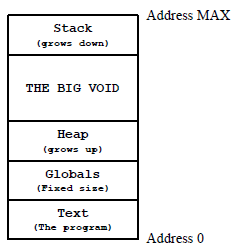
\includegraphics{sections/lec15/mem2.png}
	\end{center}
	\item \textbf{Text segment}: the code comprising a compiled program goes in the text segment.
	\item \textbf{Globals}: the compiler allocates space for any global variables
	\item \textbf{Heap}: when things are allocated via \lstinline[style=C++]{new}, they come from the heap
	\item \textbf{Stack}: stack frames are created on the stack, which grows downward
	\item \textbf{Big void}: since we don't know howbig either of these will get, we keep a big hole in between the two
	\item \textbf{Little void}: the first thousand addresses starting at zero are reserved for accidental use of as an \lstinline[style=C++]{int} as a pointer, resulting in a SEGFAULT.
\end{itemize}

\subsection{Global vs. Local vs. Dynamic}
\begin{center}
\begin{tabular}{l|l|l|l}
	& Global & Local & Dynamic \\
	\hline
	Where in code? & Outside function & Inside function (block) or args & Anywhere you use new \\
	When created? & Beginning of program & Beginning of function (block) & You call new \\
	When destroyed? & End of program & End of function & You call delete \\
	Size? & static & static & dynamic \\
	Location? & Globals & Stack & Heap \\
\end{tabular}
\end{center}
\begin{itemize}
	\item See example from lecture slides.
\end{itemize}

\subsection{Classes and dynamic memory}
\begin{itemize}
	\item When you create instances of classes, their constructors are called, just as if it were created the ``normal'' way.
\begin{lstlisting}[style=C++]
IntSet *isp = new IntSet;
\end{lstlisting}
	\begin{enumerate}
		\item Allocate enough space on the heap to hold an \lstinline[style=C++]{IntSet}
		\item Call the constructor \lstinline[style=C++]{IntSet::IntSet()} on this new object
	\end{enumerate}
\end{itemize}